%\documentclass[12pt,t]{beamer}
% \documentclass[t]{beamer}
\documentclass[handout]{beamer}\usepackage[]{graphicx}\usepackage[]{color}
%% maxwidth is the original width if it is less than linewidth
%% otherwise use linewidth (to make sure the graphics do not exceed the margin)
\makeatletter
\def\maxwidth{ %
  \ifdim\Gin@nat@width>\linewidth
    \linewidth
  \else
    \Gin@nat@width
  \fi
}
\makeatother

\definecolor{fgcolor}{rgb}{0.345, 0.345, 0.345}
\newcommand{\hlnum}[1]{\textcolor[rgb]{0.686,0.059,0.569}{#1}}%
\newcommand{\hlstr}[1]{\textcolor[rgb]{0.192,0.494,0.8}{#1}}%
\newcommand{\hlcom}[1]{\textcolor[rgb]{0.678,0.584,0.686}{\textit{#1}}}%
\newcommand{\hlopt}[1]{\textcolor[rgb]{0,0,0}{#1}}%
\newcommand{\hlstd}[1]{\textcolor[rgb]{0.345,0.345,0.345}{#1}}%
\newcommand{\hlkwa}[1]{\textcolor[rgb]{0.161,0.373,0.58}{\textbf{#1}}}%
\newcommand{\hlkwb}[1]{\textcolor[rgb]{0.69,0.353,0.396}{#1}}%
\newcommand{\hlkwc}[1]{\textcolor[rgb]{0.333,0.667,0.333}{#1}}%
\newcommand{\hlkwd}[1]{\textcolor[rgb]{0.737,0.353,0.396}{\textbf{#1}}}%
\let\hlipl\hlkwb

\usepackage{framed}
\makeatletter
\newenvironment{kframe}{%
 \def\at@end@of@kframe{}%
 \ifinner\ifhmode%
  \def\at@end@of@kframe{\end{minipage}}%
  \begin{minipage}{\columnwidth}%
 \fi\fi%
 \def\FrameCommand##1{\hskip\@totalleftmargin \hskip-\fboxsep
 \colorbox{shadecolor}{##1}\hskip-\fboxsep
     % There is no \\@totalrightmargin, so:
     \hskip-\linewidth \hskip-\@totalleftmargin \hskip\columnwidth}%
 \MakeFramed {\advance\hsize-\width
   \@totalleftmargin\z@ \linewidth\hsize
   \@setminipage}}%
 {\par\unskip\endMakeFramed%
 \at@end@of@kframe}
\makeatother

\definecolor{shadecolor}{rgb}{.97, .97, .97}
\definecolor{messagecolor}{rgb}{0, 0, 0}
\definecolor{warningcolor}{rgb}{1, 0, 1}
\definecolor{errorcolor}{rgb}{1, 0, 0}
\newenvironment{knitrout}{}{} % an empty environment to be redefined in TeX

\usepackage{alltt}
\usepackage{pgfpages}
\usepackage{pgffor}
%\pgfpagesuselayout{4 on 1}[a4paper,landscape]

%\pagestyle{empty} % descomentar para impresión muy blanca

\usepackage[utf8]{inputenc}
\usepackage[spanish]{babel}
\decimalpoint
\usepackage{verbatim}
\usepackage{hyperref}
%\hypersetup{colorlinks=false,linkbordercolor=red,linkcolor=green,pdfborderstyle={/S/U/W 1}}
%\hypersetup{colorlinks=true,linkbordercolor=red,linkcolor=green,pdfborderstyle={/S/U/W 1}}
\hypersetup{colorlinks=true,linkcolor=blue,pdfborderstyle={/S/U/W 1}}

\usepackage{amsfonts,amssymb,amsmath,amsthm, wasysym}
\usepackage{listings}
%\usepackage[T1]{fontenc}        
\usepackage{pgf}
\usepackage{epsdice}
\usepackage{pgfpages}
\usepackage{tikz}
\usetikzlibrary{arrows,shapes,plotmarks,backgrounds,trees,positioning}
\usetikzlibrary{decorations.pathmorphing,calc,snakes}
%\usepackage{marvosym}
%
\usetheme[hideothersubsections,left]{Marburg}
%\usetheme[hideothersubsections,left]{Madrid}
%\usetheme[hideothersubsections,left]{Dresden}
%\usetheme{Darmstadt}
\usecolortheme{sidebartab}
\useinnertheme[shadow]{rounded}

% \useoutertheme[footline=empty,subsection=true,compress]{infolines}
% \useoutertheme[footline=empty,subsection=true,compress]{miniframes}
% \usefonttheme{serif}

\setbeamertemplate{caption}[numbered]
%\setbeamertemplate{navigation symbols}{}
\addtobeamertemplate{navigation symbols}{}{%
    \usebeamerfont{footline}%
    \usebeamercolor[fg]{footline}%
    \hspace{1em}%
    \insertframenumber/\inserttotalframenumber
    
    \setbeamercolor{footline}{fg=blue}
\setbeamerfont{footline}{series=\bfseries}
}

\newcommand{\red}[1]{\textcolor{red}{#1}}
\newcommand{\green}[1]{\textcolor{green}{#1}}
\newcommand{\blue}[1]{\textcolor{blue}{#1}}
\newcommand{\gray}[1]{\textcolor{gray}{#1}}
\renewcommand{\emph}[1]{{\color{red}#1}}

%\newtheorem{theorem}



\setbeamertemplate{frametitle}
{\begin{centering}
\medskip
\color{blue}
\textbf{\insertframetitle}
\medskip
\end{centering}
}
\usecolortheme{rose}
\usecolortheme{dolphin}
\mode<presentation>


\newcommand{\CC}{\mathbb{C}}
\newcommand{\RR}{\mathbb{R}}
\newcommand{\ZZ}{\mathbb{Z}}
\newcommand{\NN}{\mathbb{N}}
\newcommand{\KK}{\mathbb{K}}
\newcommand{\MM}{\mathcal{M}}
%\newcommand{\dbinom}{\displaystyle\binom}

\newcommand{\limn}{{\displaystyle lim_{n\to\infty}}}

%\renewcommand{\lim}{\displaystyle \mathrm{lim}}
\renewcommand{\leq}{\leqslant}
\renewcommand{\geq}{\geqslant}
\def\tendeix{{\displaystyle\mathop{\longrightarrow}_{\scriptscriptstyle
n\to\infty}}}

\newcommand{\matriu}[1]{\left(\begin{matrix} #1 \end{matrix}\right)}

% \newcommand{\qed}{\hbox{}\nobreak\hfill\vrule width 1.4mm height 1.4mm depth 0mm
%     \par \goodbreak \smallskip}
%
% %

\theoremstyle{plain}
\newtheorem{teorema}{Teorema}
%\newtheorem{prop}{Proposición}
\newtheorem{prop}{Propiedades}
\newtheorem{cor}{Corolario}
\theoremstyle{definition}
\newtheorem{ejemplo}{Ejemplo}
\newtheorem{definicion}{Definición}
\newtheorem{obs}{Observación}

\newcounter{seccions}
\newcommand{\seccio}[1]{\addtocounter{seccions}{1}
\medskip\par\noindent\textbf{\theseccions.
#1}\smallskip\par }

\newcommand{\EM}{\Omega}
\newcommand{\PP}{\mathcal{P}}

\title[\red{Matemáticas III GINF}]{}
\author[]{R. Alberich}
\date{}
\IfFileExists{upquote.sty}{\usepackage{upquote}}{}
\begin{document}
\beamertemplatedotitem

\lstset{backgroundcolor=\color{green!50}}
\lstset{breaklines=true}
\lstset{basicstyle=\ttfamily}


\section{Variables Aleatorias Parte II}

\begin{frame}
\vfill
\begin{center}
\gray{\LARGE Variables Aleatorias Parte II}
\end{center}
\vfill
\end{frame}
\section{Variables aleatorias parte  II. Variables aleatorias continuas}


%\section{Variables aleatorias continuas}
\begin{frame}
\frametitle{Variables aleatorias continuas}


\begin{itemize}
\item Como ya hemos dicho las variables aleatorias continuas toman valores en
intervalos o áreas.
\item Lo más habitual es que estas variables tengan función de distribución continua y
derivable (salvo  a los más en una cantidad finita o numerable de puntos:-)).
\item En lo que sigue supondremos que la función de distribución de variables
aleatorias continuas cumplen estas propiedades.
\item Notemos que si $X$ es una v.a. con función de distribución continua se tiene que
$P(X=x_{0})=F_X(x_0)-F(x_0^{-})=0$. Por lo que no tiene sentido definir `'\textit{función de
probabilidad}''.
\end{itemize}
\end{frame}

\subsection{Distribuciones de probabilidad de v.a. continuas}

\begin{frame}
\begin{itemize}
\item En general tendremos que $P(X<x_0)=P(X\leq x_0)$.
\item Por otra parte podemos utilizar una regla parecida del
cociente entre casos favorables y casos posibles de Laplace  pero en
este caso el conteo se hace por la ``medida''  de los casos
posibles partida por la ``medida'' de los casos favorables.
\item Veamos un ejemplo de v.a. continua, que ampliaremos en el
tema siguiente, en el que se utilizan todos estos conceptos.
\end{itemize}
\end{frame}

\begin{frame}
\frametitle{Ejemplo: Distribución uniforme en el intervalo unidad.}

Supongamos que lanzamos un dardo a una diana de radio $1$, de forma que sea
``\textit{equiprobable}'' cualquier distancia al centro\footnote{!Cuidado! esto no es equivalente
a que cualquier punto de la diana  sea "\textit{equiprobable}":-).}.
Consideremos la v.a. continua $X=$distancia al centro.

$$F_{X}(x)=\left\{\begin{array}{ll}
0 & \mbox{si } x\leq 0\\
x & \mbox{si } 0<x<1\\
1 & \mbox{si } x\geq 1
\end{array}\right.$$
% \end{frame}
% 
% \begin{frame}
Ya que
\begin{itemize}
\item C.F. `'\textit{longitud favorable}'' $x-0$
\item C.P. `'\textit{longitud posible}'' $1-0$
\item Luego $P(X\leq x)=\frac{x-0}{1-0}=x$
\end{itemize}

\end{frame}

% \begin{frame}[fragile]
% Con el código siguiente definimos y dibujamos la función de distribución uniforme en el intervalo unidad.
% %\begin{figure}
% %\begin{center}
% %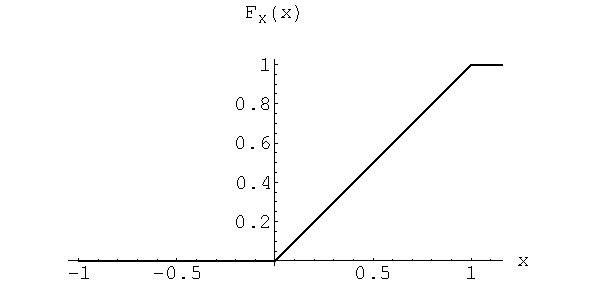
\includegraphics{distribucionuniforme}
% 
% <<echo=FALSE>>=
% curve(punif(x,0,1),xlim=c(-1,2),col="blue",main="Función de distribución de una v.a.\n uniforme en el intervalo unidad.")
% @
% %\end{center}
% %\caption{Función de distribución de una v.a. uniforme en el intervalo unidad.}
% %\end{figure}
% 
% Por ejemplo $$F_{x}(0.75)=0.75$$
% 
% \end{frame}

\begin{frame}[fragile]
\begin{figure}
\begin{center}
%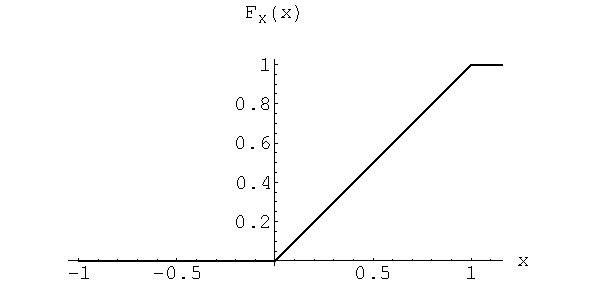
\includegraphics{distribucionuniforme}

\begin{knitrout}
\definecolor{shadecolor}{rgb}{0.969, 0.969, 0.969}\color{fgcolor}\begin{kframe}
\begin{alltt}
\hlkwd{curve}\hlstd{(}\hlkwd{punif}\hlstd{(x,}\hlnum{0}\hlstd{,}\hlnum{1}\hlstd{),}\hlkwc{xlim}\hlstd{=}\hlkwd{c}\hlstd{(}\hlopt{-}\hlnum{1}\hlstd{,}\hlnum{2}\hlstd{),}\hlkwc{col}\hlstd{=}\hlstr{"blue"}\hlstd{,}
      \hlkwc{main}\hlstd{=}\hlstr{"Función distribución uniforme."}\hlstd{)}
\end{alltt}
\end{kframe}
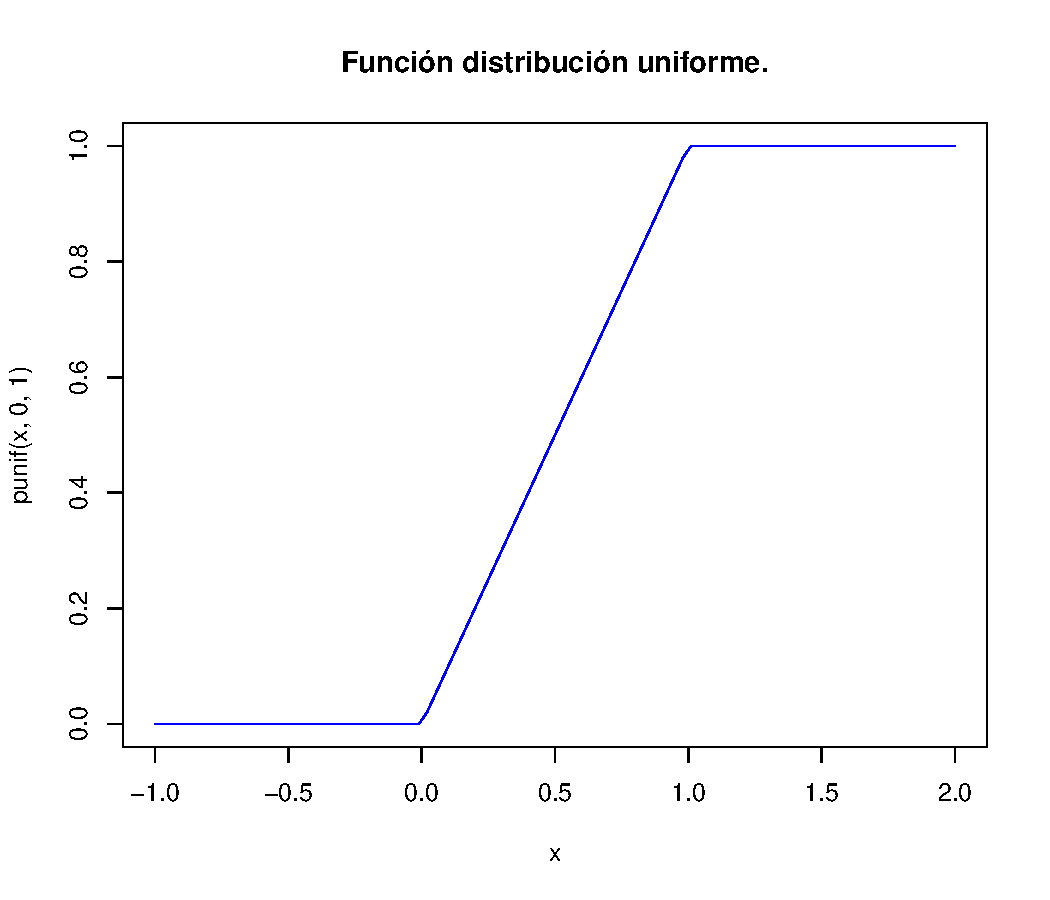
\includegraphics[width=\maxwidth]{figure/unnamed-chunk-1-1} 

\end{knitrout}

\end{center}
\caption{Función de distribución de una v.a. uniforme en el intervalo unidad.}
\end{figure}


\end{frame}


\begin{frame}
En las variables continuas los sucesos del tipo $\{X\leq x \}$ y $\{X< x \}$ tendrán la
misma probabilidad, y otros tipos de sucesos similares también, algunas de estas
propiedades se explicitan en la siguiente proposición.

\begin{prop}
Dada una v.a. continua $X$ se tiene que:
\begin{enumerate}[a)]
\item $P(X\leq b)=P(X<b)$
\item $P(X<b)=P(X<a)+P(a<X<b)$
\item $P(a<X<b)=P(X<b)-P(X<a)$
\end{enumerate}
\end{prop}
\end{frame}


\begin{frame}
\textbf{Demostración:}
\begin{itemize}
\item[b)] $\{X<a\}\cap \{a<X<b\}=\emptyset$
$\{X<a\}\cup \{a<X<b\}=\{X<a\}$ entonces
\begin{equation*}
\begin{split}
P(X\leq b)= & P(\{X<a\}\cup \{a<X<b\})\\
& = P(X<a)+P(a<X<b)
\end{split}
\end{equation*}

\item[a)] $P(X<b)=P(X<b)+P(X=b)=P(X<b)$
\item[c)] \'Idem que b) aplicando a).
\end{itemize}
\end{frame}

\begin{frame}
Las propiedades anteriores  y combinaciones de ellas se pueden
escribir utilizando la función de distribución de $X$:

\begin{prop}Dada una variable aleatoria continua se tiene que:
\begin{enumerate}[a)]
\item $F_{X}(b)=F_{X}(a)+P(a<X<b)$
\item $P(a<X<b)=F_{X}(b)-F_{X}(a)$
\item $P(a\leq X\leq b)=F_{X}(b)-F_{X}(a)$
\end{enumerate}
\end{prop}
\end{frame}

\begin{frame}
\textbf{Demostración:} ejercicio.

\frametitle{Ejemplo}
En los dardos:
$$P(0.25<X<0.3)=F_{X}(0.3)-F_{X}(0.25)=$$
$$=0.3-0.25=0.05$$

\end{frame}


\subsection{Función de densidad}
\begin{frame}
Una función $f:\RR\to\RR$ es una función de densidad sobre $\RR$ si cumple que

\begin{enumerate}[a)]
\item $f_{X}(x)\geq 0$ para todo $x \in\RR.$
\item $f$ es continua salvo a lo más en una cantidad finita de puntos sobre
cada intervalo acotado de $\RR$.
\item $\int\limits_{-\infty}^{+\infty} f_{X}(x) dx=1.$
\end{enumerate}
\end{frame}




\begin{frame}
\begin{definicion}
Sea $X$ una v.a. con función de distribución $F_X$. Sea $f:\RR\to\RR$ una función de
densidad tal que
$$F_X(x)=\int_{-\infty}^{x} f_X(t) dt.\mbox{ para todo } x\in\RR.$$

Entonces $X$ es una variable aleatoria continua y $f_X$ es la densidad de la v.a.  $X$.

El conjunto $D_X=\{x\in\RR| f_x(x)>0\}$ recibe el nombre de soporte o dominio de la
variable aleatoria continua y se interpreta su conjunto de resultados posibles.
\end{definicion}
\end{frame}

\begin{frame}

En nuestra diana la función $f$ es una densidad
$$f_{X}(x)=\left\{
\begin{array}{ll}
0 & \mbox{si } x\leq 0\\
1 & \mbox{si } 0 < x < 1\\
0 & \mbox{si } 1\leq x
\end{array}\right.
$$
\end{frame}

\begin{frame}
que    es la densidad de $X$, en efecto:

\begin{itemize}
\item Si $x \leq 0$ entonces $\int_{-\infty}^x f_X(t) dt = 0.$
\item  Si $0\leq x\leq 1$ entonces $\int_{-\infty}^x f_X(t) dt =
\int_{0}^x 1 dt = x.$
\item Si $x\geq 1$  entonces $\int_{-\infty}^x f_X(t) dt =
\int_{0}^1 1 dt = 1.$
\end{itemize}

Por lo tanto  $F_X(x)=\int_{-\infty}^x f_X(t) dt$ para todo $x\in\RR.$
\end{frame}

\begin{frame}[fragile]

\begin{figure}
\begin{center}
%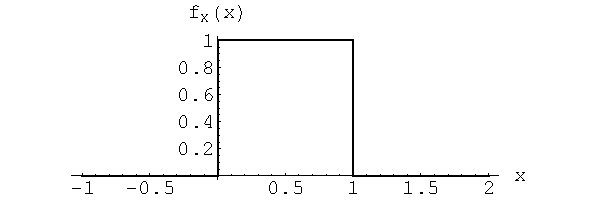
\includegraphics{densidaduniforme}
\begin{knitrout}
\definecolor{shadecolor}{rgb}{0.969, 0.969, 0.969}\color{fgcolor}\begin{kframe}
\begin{alltt}
\hlkwd{curve}\hlstd{(}\hlkwd{dunif}\hlstd{(x,}\hlnum{0}\hlstd{,}\hlnum{1}\hlstd{),}\hlkwc{xlim}\hlstd{=}\hlkwd{c}\hlstd{(}\hlopt{-}\hlnum{0.5}\hlstd{,}\hlnum{1.5}\hlstd{),}\hlkwc{col}\hlstd{=}\hlstr{"blue"}\hlstd{,}
      \hlkwc{main}\hlstd{=}\hlstr{"Densidad uniforme"}\hlstd{)}
\end{alltt}
\end{kframe}
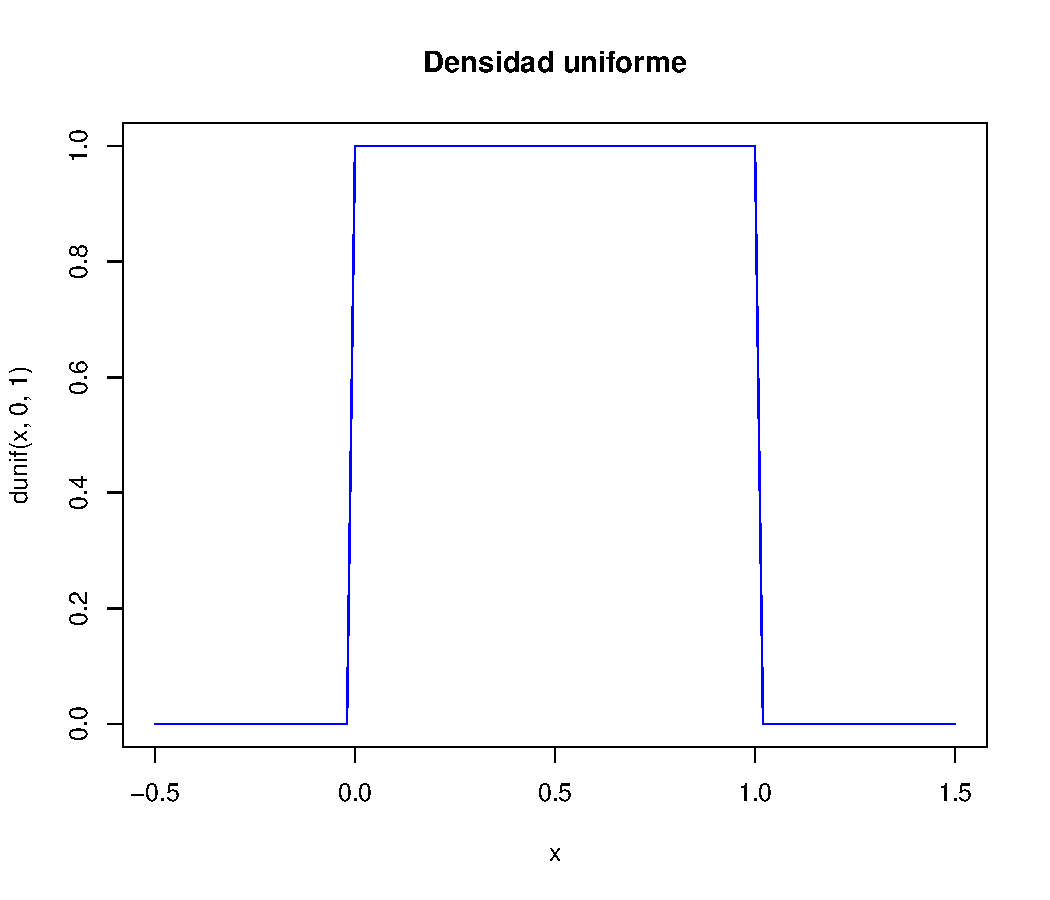
\includegraphics[width=\maxwidth]{figure/unnamed-chunk-2-1} 

\end{knitrout}
\end{center}
\caption{Función de densidad de una v.a. uniforme en el intervalo
$(0,1)$}
\end{figure}

\end{frame}

\begin{frame}
La función de densidad nos permite calcular diversas probabilidades.

\begin{prop} Sea $X$ una v.a. continua con función de distribución $F_X$ y de
densidad $f_X$, entonces
\begin{enumerate}[a)]
\item \begin{equation*}
\begin{split}
P(a< X< b)= & P(a<X\leq b)= P(a\leq X< b)\\
= &  P(a\leq X\leq b)= \int_{a}^b f_X(x) dx.
\end{split}
\end{equation*}
\item Si $A$ es un conjunto  adecuado de $\RR$
entonces $P(X\in A)=\int_{A} f(x) dx=\int_{A\cap D_X} f(x) dx$.
\end{enumerate}
\end{prop}
\end{frame}


\begin{frame}

\begin{prop}
Sea $X$ una v.a. continua con función de distribución $F_X$ y de densidad $f_X$, entonces:

\begin{enumerate}[a)]
\item Si $f_x$ es continua en un punto $x$, $F_X$ es derivable en ese punto y
$F_X'(x)=f_X(x).$
\item $P(X=x)=0$ para todo $x\in\RR.$
\end{enumerate}
\end{prop}
\end{frame}
%%%  \textbf{Ejercicio:} Comprobar estas propiedades en la diana.



\begin{frame}
\frametitle{Ejemplo}
Sea $X=$ tiempo de ejecución de un proceso. Se supone que $X$
sigue una distribución uniforme en dos unidades de tiempo,
si tarda más el proceso se cancela. Entonces

$$F_{X}(x)=P(X\leq x)=\frac{CF}{CP}=\frac{x}{2}$$
Luego su función de distribución es:



$$F_{X}(x)=\left\{\begin{array}{ll}
0 & \mbox{si } x\leq 0\\
\frac{x}{2} & \mbox{si } 0<x<2\\
1 & \mbox{si } 2\leq x
\end{array}\right.$$
\end{frame}

\begin{frame}
mientras que su función de densidad es:
$$f_{X}(x)=F_{X}'(x)=\left\{\begin{array}{ll}
0 & \mbox{si } x\leq 0\\
\frac{1}{2} & \mbox{si } 0<x\leq 2\\
0 & \mbox{si } 2\leq x
\end{array}\right.$$

Efectivamente
\begin{itemize}
\item $f_{X}(x)\geq 0,$ y tiene un conjunto finito de discontinuidades.
\item $F_X(x)=\int_{-\infty}^x f_X(t) dt.$ para todo $x\in \RR$ (ejercicio,
resolverlo gráficamente.)
\item $\int\limits_{-\infty}^{+\infty}f_{X}(x)dx=
\int\limits_{0}^{2}\frac{1}{2}dx=\frac{x}{2}\mid_{0}^{2}=
=\frac{2}{2}-\frac{0}{2}=1.$
\end{itemize}
\end{frame}

\begin{frame}
\textbf{Ejercicio:} Calcular la probabilidad de que uno de nuestros procesos tarde
más de una unidad de tiempo en ser procesado. Calcular también la  probabilidad de
que dure entre $0.5$ y $1.5$ unidades de tiempo.
\end{frame}
\section{Momentos para variables aleatorias continuas}
\begin{frame}
Los mismos comentarios y definiciones que se dieron en la sección correspondiente del tema
de estadística descriptiva %\ref{modis}
son aplicables aquí. Así que sólo daremos las
definiciones, la forma de cálculo y algunos ejemplos.
\end{frame}

\subsection{Esperanza de  una v.a. continua}


\begin{frame}
Sea $X$ una v.a. continua con función de densidad $f_{X}(x)$
entonces:

\begin{itemize}
\item su esperanza es :
$E(X)=\int\limits_{-\infty}^{+\infty} xf_{X}(x)dx.$
\item Si $g(x)$ es una función de la variable $X$ entonces
$$E(g(X))=\int\limits_{-\infty}^{+\infty} g(x)f_{X}(x)dx.$$
\end{itemize}
\end{frame}

\subsection{Varianza  de una  v.a. continuas}

\begin{frame}
\begin{itemize}
\item $Var(X)=\sigma_{X}^{2}=E((X-\mu_{X})^2)=
\int\limits_{-\infty}^{+\infty} (x-\mu_{X})^2 f_{X}(x)dx.$
\item A $\sigma_{X}=+\sqrt{\sigma_{X}^{2}}$ se le denomina desviación típica  de $X$.
\end{itemize}
\end{frame}
\begin{frame}



\textbf{Propiedades}
\begin{itemize}
\item $\sigma_{X}^{2}\geq 0$
\item $Var(cte)=E(cte^2)-(E(cte))^2= cte^2 - cte^2=0$
\item $Var(x)=E(X^{2})-\mu_{X}^2=\int\limits_{-\infty}^{+\infty}x^2
f_{X}(x)dx - \mu_{X}^2.$
\item El mínimo de $E((X-C)^2)$ se alcanza cuando $C=E(X)$ y es $Var(X)$.
\end{itemize}
\end{frame}

\begin{frame}

\textbf{Ejemplos} Calcular $\mu_{X}$ y $\sigma_{X}^{2}$ en el dardo.

Resultado $\mu_{X}=\frac{1}{2}$, $E(X^2)=\frac{1}{3}$,
$Var(X)=\frac{1}{12}$.
\end{frame}
%\section{Transformación de variables aleatorias}
\subsubsection{Esperanza y varianza de trasformaciones lineales}


\begin{frame}
Sea $X$ una v.a. continua con $E(X)=\mu_{X}$ y $Var(X)=\sigma_{X}^{2}$ sea $Y=a+b X$, donde
$a,b\in\RR$, es una nueva v.a. continua obtenida mediante una transformación lineal de $X$.
Se verifican las mismas propiedades que en el caso discreto:
\begin{itemize}
\item  $E(Y)=E(a+b X)=a+b E(X)$
\item $Var(Y)=Var(a+b X)=b^{2} Var(X)$
\item $\sigma_{Y}=|b| \sigma_{X}$
\item $Z=\frac{X-\mu_{X}}{\sigma_{X}}$ es una transformación
lineal de $X$ de forma que
$$E(Z)=0 \mbox{ y } Var(Z)=1$$
\end{itemize}
\end{frame}

\begin{frame}

\textbf{Ejemplo}
En una empresa de venta de vinos por internet, sea
$X=$ número de  litros de vino del país vendidos en un año.
Supongamos que sabemos que $E(X)=10000$ y que $Var(X)=100$
Supongamos que los gastos fijos de distribución son
50000 y el beneficio por litro es de 10 pts por botella.
Definimos $T=10 X-50000$ que será el beneficio después de gastos
entonces:
$$E(T)=10 E(X)-50000 = 50000$$
y
$$Var(T)=10^2 VAR(X)= 10000$$

\end{frame}
\section{Transformación de variables aleatorias}
\begin{frame}


Muchas variables aleatorias son funciones de otras v.a. En lo que
sigue resumiremos diversas técnicas para dada una v.a. $X$ y una
transformación $Y=h(X)$  encontrar $F_{Y}$ a
partir de $F_{X}$.

\end{frame}
\subsection{Transformaciones de v.a. discretas}


\begin{frame}


\begin{prop}
Sea $X$ una v.a. discreta con \newline
$X(\Omega)=\{x_{1},x_{2},\ldots,x_{n},..\}$ y sea $h:\RR\to\RR$ una aplicación.
Entonces $Y=h(X)$ es también una v.a. discreta. Además si $P_X$
y $F_{X}$ son las funciones de probabilidad y de distribución de
$X$ entonces

\begin{enumerate}[a)]
\item $\displaystyle P_{Y}(y)=\sum_{x_{i}|h(x_{i})=y}P_X(x_{i}).$
\item $\displaystyle F_{Y}(y)=\sum_{x_{i}|h(x_{i})\leq y} P_X(x_{i}).$
\end{enumerate}
\end{prop}
\end{frame}
\subsection{Transformaciones de v.a. continuas}



\begin{frame}



Desafortunadamente este caso no es tan sencillo como el anterior, pues la
transformación de una v.a. continua puede ser continua, discreta, mixta \ldots

\begin{prop}
Sea $X$ una v.a. continua cuya función de densidad es $f_{X}$. Sea
$h:\RR\to\RR$ una aplicación estrictamente monótona y derivable, tal
que $h'(x)\not=0$ para todo $x\in\RR$. Sea $Y=h(X)$ la
transformación de $X$ por $h$. Entonces $Y$ es una v.a. continua con función
de densidad

$$f_{Y}(y)=\left.\frac{f_{X}(x)}
{\left|h'(x)\right|}\right|_{x=h^{-1}(y)}$$
\end{prop}
\end{frame}

\begin{frame}

\begin{prop}
Sea $X$ una v.a. continua cuya función de densidad es $f_{X}$. Si
$h:\RR\to\RR$ es  una aplicación, no necesariamente monótona,
pero sí derivable con derivada no nula, y si
la ecuación $h(x)=y$ tiene un número finito de soluciones
$x_{1},x_{2},..,x_{n}$ entonces:

$$\displaystyle f_{Y}(y)=\left.\sum_{k=1}^{n} \frac{f_{X}(x)}
{\left|h'(x)\right|}\right|_{x=x_{k}}$$
\end{prop}
\end{frame}
\subsubsection{Método general}
\begin{frame}


Cuando no podamos aplicar las propiedades anteriores intentaremos
calcular primero la función de distribución de la transformación
y luego su densidad.

Notemos que en general si $Y=g(X)$ es una v.a. transformación  de la
v.a. $X$ entonces

$$F_{Y}(y)=P(Y\leq y)=P(g(X)\leq y)$$

Por ejemplo si $g$ es estrictamente creciente y cont.

$$F_{Y}(y)=P(g(X)\leq y)=P(X\leq g^{-1}(y))=F_{X}(g^{-1}(y))$$

y si $g$ es estrictamente decreciente y cont.
$$F_{Y}(y)=P(g(X)\leq y)=P(X\geq g^{-1}(y))=1-F_{X}(g^{-1}(y))$$

\end{frame}
\section{Desigualdad de Chebyshef}
\begin{frame}


\begin{itemize}
\frametitle{Desigualdades de Markov y de Chebyshef}
\item Veremos en esta sección distintas desigualdades que acotan determinadas probabilidades de
una variable aleatoria.
\item Estas desigualdades sirven en algunos casos para acotar
probabilidades de determinados sucesos.
\item También son útiles desde el punto de vista
teórico, por ejemplo para justificar que la varianza es una mediada de la dispersión de
los datos.
\end{itemize}
\end{frame}

\subsection{Desigualdad de Markov}
\begin{frame}

\begin{prop}
Sea $X$ una v.a. positiva con $E(X)$ finita. Entonces
$P(X\geq a)\leq \frac{E(X)}{a}$ para todo $a>0$.
\end{prop}
\end{frame}

\begin{frame}

\textbf{Demostración: }

Si $X$ es continua  y sólo toma valores positivos\newline
\begin{equation*}
\begin{split}
E(X)=& \int_{-\infty}^{+\infty} x f_{X}(x) dx=  \int_{0}^{+\infty} x f_{X}(x) dx\\
= & \displaystyle \int_{0}^{a} x f_{X}(x)
dx+\int_{a}^{+\infty} x f_{X}(x) dx \\
\geq &  \int_{a}^{+\infty} x
f_{X}(x) dx \geq\displaystyle a \int_{a}^{+\infty}
f_{X}(x) dx\\
=& a\cdot  P(X\geq a)
\end{split}
\end{equation*}

de donde se sigue que  
$$P(X\geq a)\leq \frac{E(X)}{a}.$$
\end{frame}

\begin{frame}

\begin{prop}
Sea $X$ una v.a. con $E(X)$ finita entonces  para todo $a>0$

$$P(|X|\geq a )\leq
\frac{E(|X|)}{a}$$
\end{prop}

\end{frame}
\subsubsection{Desigualdad de Chebyshef}
\begin{frame}


\begin{prop}
Sea  $X$ una v.a.con $E(X)=\mu$ y $Var(X)=\sigma^2$ 
entonces para todo $a>0$

$$P(|X-\mu|\geq a)\leq \frac{\sigma^{2}}{a^2}$$ 
\end{prop}

\end{frame}

\begin{frame}

\textit{Demostración}:

Apliquemos la consecuencia de la desigualdad de Markov a la v.a.
no negativa 

$$Y^2=(X-\mu)^{2}$$

entonces
\begin{equation*}
\begin{split}
P(Y^2\geq a^2)\leq & 
\frac{E(Y^2)}{a^2}=\frac{E((X-\mu)^{2})}{a^2}\\
= & \frac{Var(X)}{a^2}=\frac{\sigma^{2}}{a^{2}}
\end{split}
\end{equation*}

\end{frame}

\begin{frame}

Por otra parte

$$P(Y^2\geq a^2)=P(|Y|\geq a)= P(|X-\mu|\geq a)$$

hecho que, junto con la desigualdad anterior,
demuestra el resultado.

\end{frame}

\begin{frame}


\textbf{Observación:} Supongamos que $X$ es una v.a. con $Var(X)=0$
entonces.


Aplicando la desigualdad anterior

$$P(|X-E(X)|\geq a )=0$ para todo $a>0$$ 
lo que implica que

$$P(X=E(X))=1$$

Por lo que  probabilidad de que $X$ sea
constantemente $E(X)$ es 1.

Lo que nos confirma la utilidad de la varianza es una
medida de la dispersión de los datos.
\end{frame}

\begin{frame}

\frametitle{Ejemplo}

Se sabe que el tiempo de respuesta medio y la desviación típica de
un sistema multiusuario  son 15 y 3 u.t.
respectivamente. Entonces:

$$P(|X-15|\geq 5)\leq \frac{9}{25}=0.36.$

Si substituimos $a$ por $a\cdot \sigma$ en la
desigualdad de Chebyshef. 
\end{frame}

\begin{frame}

Nos queda:

$$P(|X-\mu|\geq a \sigma)\leq
\frac{\sigma^2}{(a\sigma)^2}=\frac{1}{a^2}.$$

Que es otra manera de expresar la desigualdad de Chebyshef.

La desigualdad de Chebyshef también se puede escribir de al menos dos maneras más:

$$P(\mu-a\leq X\leq \mu+a)\geq 1-\frac{\sigma^2}{a^2}$$

$$P(\mu-a\cdot \sigma\leq X\leq \mu+ a \cdot \sigma)$$
%
\end{frame}

\subsubsection{La varianza como medida de dispersión}
\begin{frame}
Tomando la segunda expresión que hemos visto para la desigualdad de
Chebyshef para distintos valores de $a>0$ tenemos la siguiente tabla.
\begin{center}
\begin{tabular}{l|l}
a & $P(|X-E(X)|\geq a \sigma)$\\
\hline
1 & $\leq 1$ \\
2 & $\leq 0.25$ \\
3 & $\leq 0.111$ \\
4 & $\leq 0.0025$
\end{tabular}
\end{center}

\end{frame}

\begin{frame}[fragile]
\frametitle{Interpretación de la desigualdad}
\begin{itemize}
\item Por ejemplo para $a=2$ esta desigualdad se puede interpretar como 
que dada una v.a. $X$ con cualquier distribución
que tenga $E(X)$ y $Var(X)$ finitos
\emph{la  probabilidad de que un valor se aleje de la media $\mu$ más de
$a=2$ desviaciones típicas es menor o igual que $0.25$}.
\item Es decir sólo el 25\% de los valores estarán alejados de la media
más de $2\sigma$

¡\emph{Sea cual sea la distribución de la v.a.}!
\end{itemize}
\end{frame}


\end{document}
